\documentclass[acmtog]{acmart}
\usepackage{graphicx}
\usepackage{subfigure}
\usepackage{natbib}
\usepackage{listings}
\usepackage{bm}
\usepackage{amsmath}
\usepackage{verbatim}

\definecolor{blve}{rgb}{0.3372549, 0.61176471, 0.83921569}
\definecolor{gr33n}{rgb}{0.29019608, 0.7372549, 0.64705882}
\makeatletter
\lst@InstallKeywords k{class}{classstyle}\slshape{classstyle}{}ld
\makeatother
\lstset{language=C++,
	basicstyle=\ttfamily,
	keywordstyle=\color{blve}\ttfamily,
	stringstyle=\color{red}\ttfamily,
	commentstyle=\color{magenta}\ttfamily,
	morecomment=[l][\color{magenta}]{\#},
	classstyle = \bfseries\color{gr33n}, 
	tabsize=2
}
\lstset{basicstyle=\ttfamily}

% Title portion
\title{Assignment 2 : Geometric Modeling}

\author{Name:\quad Entropy-Fighter\\ student number:\ 2020533
\\email:\quad xxxx@shanghaitech.edu.cn}

% Document starts
\begin{document}
\maketitle

\vspace*{2 ex}

\section{Introduction}
\quad In Assignment2, we are required to draw bezier curve and bezier surface.
In this homework, I do the following things.
\begin{itemize}
\item (must)Use some algorithms to implement the bezier curve.
\item (must)Use some algorithms to implement the bezier surface.
\item (must)Generate objects and render the bezier surface using phong lighting model.
\item (must)Use information in the "tea.bzs" file to patch together multiple bezier surfaces.
\item (optional)Use some algorithms to implement the bspline curve and bspline surface, and render them.
\item (optional)Implement the interactive editing (by selection) of control points by using mouse.
\end{itemize}
\section{Implementation Details}
\subsection{Evaluating points on Bézier curve with De Casteljau's Algorithm}
\quad This part is implemented in the bezier curve's "evaluate" function in "bezier.cpp". I use De Casteljau's Algorithm to 
solve this problem.
The pseudo code for the De Casteljau's Algorithm is shown below.
\begin{lstlisting}
	Input: array P[0:n] of n+1 points 
	and real number u in [0,1]	
	Output: point on curve, C(u)
	Working: point array Q[0:n] (the point
	has 2 attributes: pos and normal)
	
	for i := 0 to n do
		Q[i] := P[i]; // save input
	for k := 1 to n do
		for i := 0 to n - k do
			if k == n - 1
        	Q[0].normal = \
				normalize(Q[1].normal - Q[0].normal);
			Q[i].pos := \
			(1 - u) * Q[i].pos + u * Q[i + 1].pos;
	return Q[0];
\end{lstlisting}
\subsection{Constructing the Bézier surface}
\quad This part is implemented in the bezier surface's "evaluate" function in "bezier.cpp". Since we have known how to evaluate points on the bezier curve, it is quite easy to evalute points on the bezier surface. 
It just changes from 2D to 3D. The basic idea to solve the problem is to fix one direction and apply the de Casteljau algorithm to another direction.
Note that I get the point's normal from the cross product of the 2 tangent vectors of different directions. The pseudo code of this process is shown below.
\begin{lstlisting}
	Input: m+1 rows and n+1 columns \
	of control points and (u,v).
	Output: point on surface p(u,v)
	Algorithm:

	for i := 0 to m do
	begin
		Apply de Casteljau algorithm to \
		the i-th row of control points with v;
		Let the point obtained be q_i(v);
	end
	Apply de Casteljau algorithm \
	to q_0(v), q_1(v), ..., q_m(v) with u;
	The point obtained is p(u,v);
\end{lstlisting}

\subsection{Rendering the Bézier surfaces}
\quad 
After evaluating the points to the surface, we begin to generate the objects. 
This part is implemented in the bezier surface's "generateObject" function in "bezier.cpp". 
I just do the uniform sampling in this part. 
Given any (u,v) ranging from [0,1]*[0,1], 
I use the algorithm demonstrated above to sample some points on the surface.

Then I store the points' information in the vertex array, and fill indices to the indices array which stores the sequence of points to construct triangle meshes.

The rest part is the same as the work done in hw1. We need to design the shaders and apply the phong lighting model. Also, we need to deal with VBO, VAO and EBO. 

\subsection{Patching together multiple Bézier surfaces}
\quad This part is implemented in the "read" function in "bezier.cpp". 
When we are patching together multiple bézier surfaces, we should make sure that the edge to be soft, which means the new surface should still maintain 1st order continuity. 

In order to achive this, there are 2 rules to obey. Firstly, the points on the edge are connected. Secondly, their tangent vectors on the edge should be continuous. 
This can be done by setting the control points properly by hands. 

Fortunately, the teaching group has offered us the "tea.bzs" file. 
In the "tea.bzs", b represents the number of Bézier surfaces, p represents the number of control points, m and n represent the row and column numbers of the Bézier surface's control points. For each bezier surface, we store the control points information. Then, we store the bezier surfaces to the big vector. 

After reading the information from the file, we just need to draw and render all these different bezier surfaces.

\subsection{(Optional)Constructing the Bspline surface}
\quad This part is implemented in "bspline.cpp". The schema of "bspline.cpp" is similar to that of "bezier.cpp", containing both the BsplineCurve class and BsplineSurface class.

Like De Casteljau's Algorithm used in section 2.1, we use De Bool's Algorithm to evaluate the points on the bspline curve. The pseudo code for the De Bool's Algorithm is shown below.
\begin{lstlisting}
	Input: a value u
	Output: the point on the curve, C(u)
	
	If u lies in [u_k,u_(k+1)) \
	and u != u_k: \
	h = p (inserting u in (p) times) \
	and s = 0;
	If u = u_k and u_k is \
	a knot of multiplicity s: \
	h = p - s (inserting u in (p - s) times);
	Copy the related control points \
	P_(k-s), P_(k-s-1), P_(k-s-2), \
	..., P_(k-p+1) and P_(k-p) \
	to a new array and rename them as \
	P_(k-s,0), P_(k-s-1,0), \
	P_(k-s-2,0), ..., P_(k-p+1,0);
	
	for r := 1 to h do
		for i := k-p+r to k-s do
		begin
			a_(i,r) = (u - u_i) / ( u_(i+p-r+1) - u_i )
			P_(i,r) = (1 - a_(i,r)) * P_(i-1,r-1) \
			+ a_(i,r) * P_(i,r-1)
		end
	P_(k-s,p-s) is the point C(u).
\end{lstlisting}
\quad Then it's quite easy to evaluate the point on B-spline surface based on De Boor's algorthm. 
The procedure is almost the same as that in section 2.2. 
The process is shown below in pseudo code. 
\begin{lstlisting}
Input: a set of m+1 rows and n+1 
columns of control points, 
knot vectors in the u- and v-directions 
and (u,v);
Output: point on the surface p(u,v)
Algorithm:

Let u be in [u_c,u_(c+1));
Let v be in [v_d,v_(d+1));
If u is not equal to u_c, let s be zero; 
otherwise, let s be the multiplicity of u_c;
If v is not equal to v_d, let t be zero; 
otherwise, let t be the multiplicity of v_d;
for i := c-p to c-s do
	begin
		Apply de Boor algorithm to control points \
		p_(i,d-q), p_(i,d-q+1), ..., p_(i,d-t) \
		with respect to v;
		Let the result be q_i(v);
	end
Apply de Boor algorithm to points \
q_(c-p)(v), q_(c-p+1)(v), ..., q_(c-s)(v) \
with respect to u;
The point obtained is p(u,v);
\end{lstlisting}

The rest work is the same as the section 2.3. 

In general, I learn these algorithms from the website \\
 https://pages.mtu.edu/~shene/COURSES/cs3621/NOTES. 
However, the algorithms seem a bit different from the content in course slide's bspline part. Therefore, I do some math proof.
\begin{figure}[h]
	\centering
	{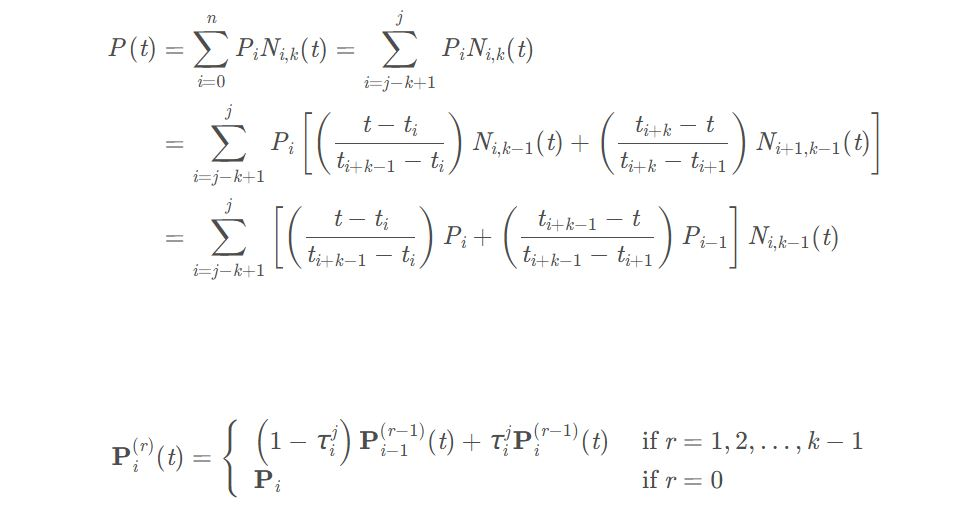
\includegraphics[width=6cm]{math.JPG}}	
\end{figure}
\subsection{(optional)Interactive editing (by selection) of control points}
\quad This part is implemented in the "processInput" function and the rendering loop in "main.cpp". 
Firstly, I render many white little cubes to represent control points. This is the most easy part in this section. Then, I deal with some complex problems below. 

To implement the interactive editing (by selection) of control points,
my basic idea is to get the world coordinate of my cursor. However, without knowing the depth of the objects, I cannot find the coordinate and can only get all the coordinates on the view direction. 
Fortunately, I search on the stackoverflow website, and find that glReadPixels function is useful enough to get the depth! Also, glm::unproject() is useful enough to change from screen coordinate to world coordinate!

Therefore, I can get the world coordinate of my cursor easily! 
Then, I just compare this position to all control points' positions to get the closest control point's positions.
After thet, I update the control point's position to wherever I move the mouse. Also, I update the corresponding surface objects.
After doing all of these, I get an interactive bezier surface!
\section{Results}
% pictures should be in
\quad The first left picture is all the rendered elements.

The second left picture is the single bezier surface.

The third left picture is the tea objects, which is composed by multiple bezier surfaces.


The first right picture is the bspline surface.

The second right picture is the bezier surface before interactive dragging.

The third right picture is the bezier surface after interactive dragging.
\begin{figure}[h]
	\centering
	{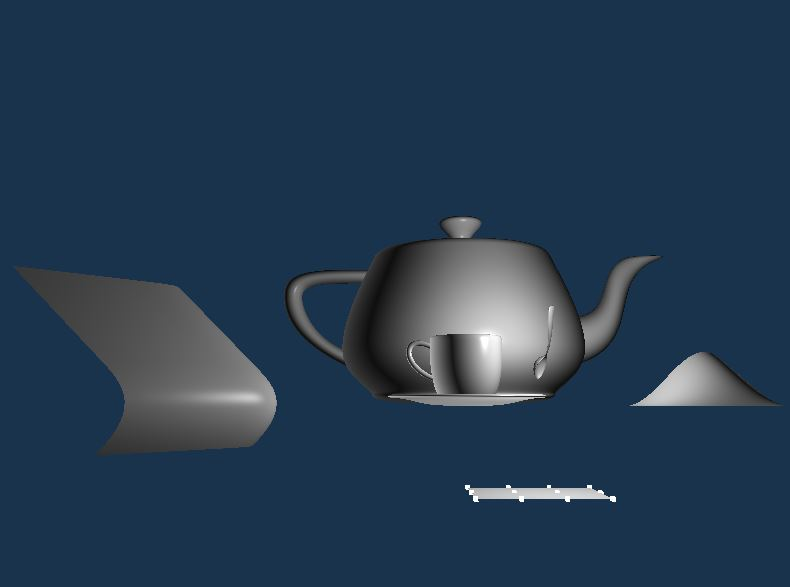
\includegraphics[width=8cm]{all_elements.JPG}}	
	{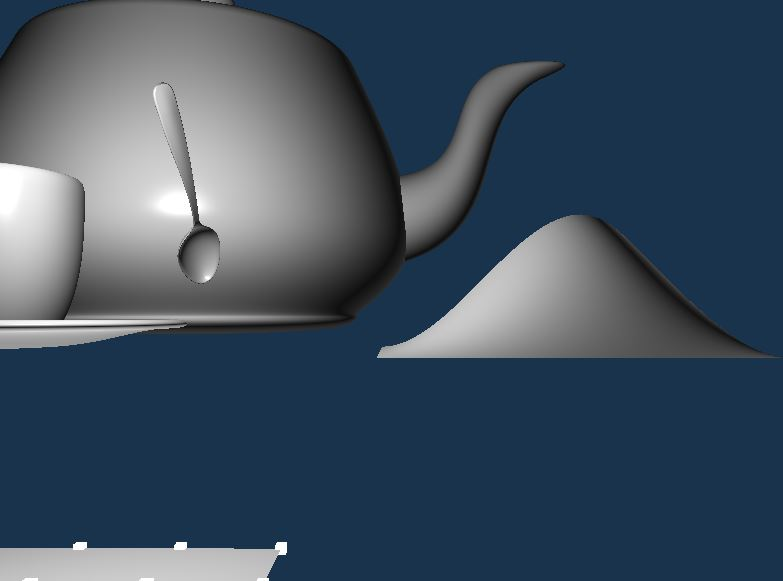
\includegraphics[width=8cm]{single_bezier.JPG}}
	{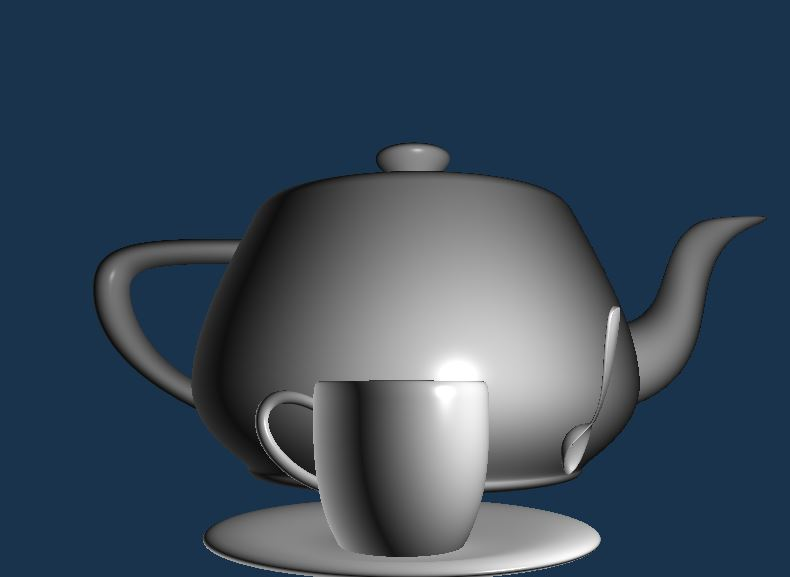
\includegraphics[width=8cm]{tea.JPG}}
\end{figure}
\begin{figure}[h]
	\centering
	{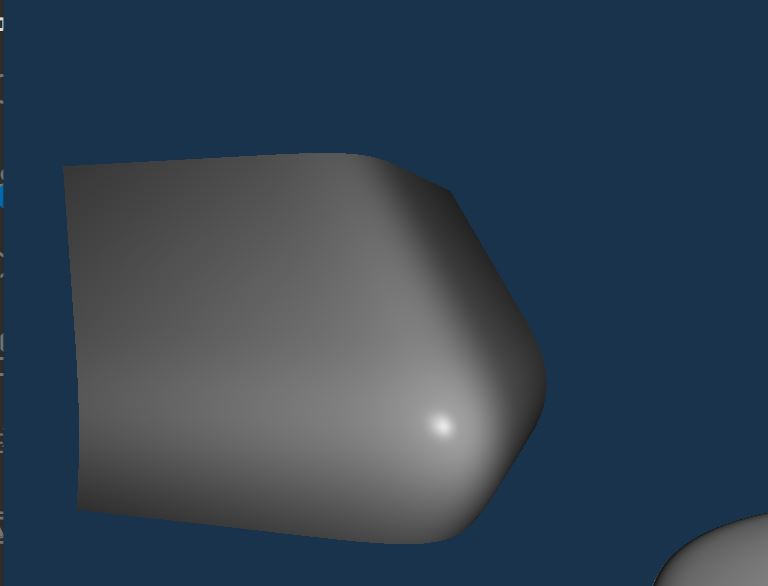
\includegraphics[width=8cm]{bspline.JPG}}
	{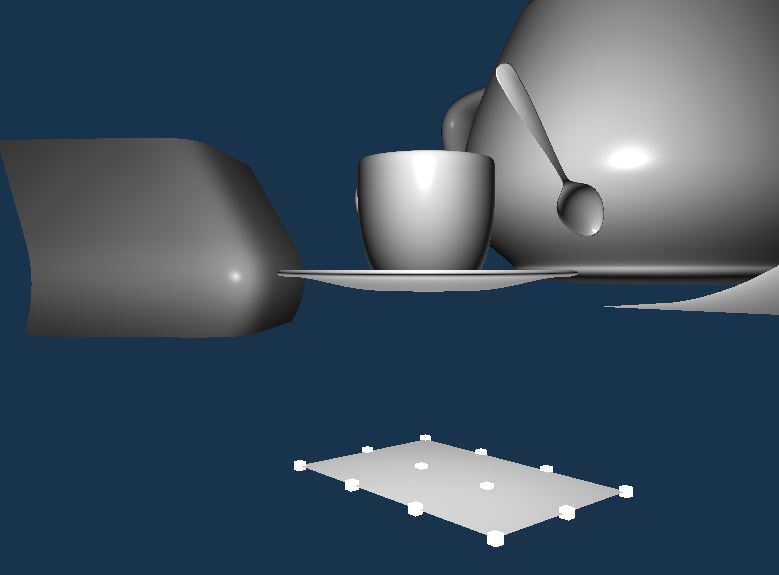
\includegraphics[width=8cm]{interactive1.JPG}}
	{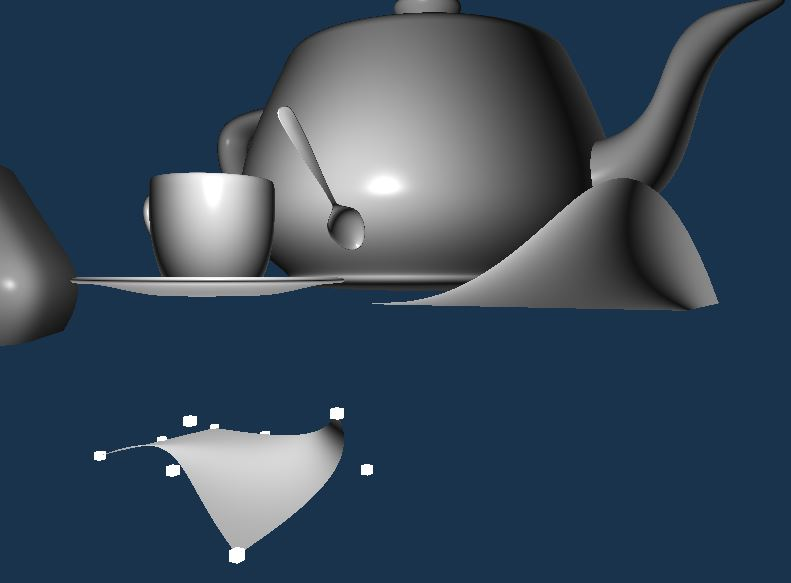
\includegraphics[width=8cm]{interactive2.JPG}}
\end{figure}
\end{document}
